% Options for packages loaded elsewhere
\PassOptionsToPackage{unicode}{hyperref}
\PassOptionsToPackage{hyphens}{url}
\PassOptionsToPackage{dvipsnames,svgnames,x11names}{xcolor}
%
\documentclass[
  11pt,
  a4paper,
  DIV=11,
  numbers=noendperiod]{scrartcl}

\usepackage{amsmath,amssymb}
\usepackage{iftex}
\ifPDFTeX
  \usepackage[T1]{fontenc}
  \usepackage[utf8]{inputenc}
  \usepackage{textcomp} % provide euro and other symbols
\else % if luatex or xetex
  \usepackage{unicode-math}
  \defaultfontfeatures{Scale=MatchLowercase}
  \defaultfontfeatures[\rmfamily]{Ligatures=TeX,Scale=1}
\fi
\usepackage{lmodern}
\ifPDFTeX\else  
    % xetex/luatex font selection
\fi
% Use upquote if available, for straight quotes in verbatim environments
\IfFileExists{upquote.sty}{\usepackage{upquote}}{}
\IfFileExists{microtype.sty}{% use microtype if available
  \usepackage[]{microtype}
  \UseMicrotypeSet[protrusion]{basicmath} % disable protrusion for tt fonts
}{}
\makeatletter
\@ifundefined{KOMAClassName}{% if non-KOMA class
  \IfFileExists{parskip.sty}{%
    \usepackage{parskip}
  }{% else
    \setlength{\parindent}{0pt}
    \setlength{\parskip}{6pt plus 2pt minus 1pt}}
}{% if KOMA class
  \KOMAoptions{parskip=half}}
\makeatother
\usepackage{xcolor}
\usepackage[margin=2cm]{geometry}
\setlength{\emergencystretch}{3em} % prevent overfull lines
\setcounter{secnumdepth}{-\maxdimen} % remove section numbering
% Make \paragraph and \subparagraph free-standing
\ifx\paragraph\undefined\else
  \let\oldparagraph\paragraph
  \renewcommand{\paragraph}[1]{\oldparagraph{#1}\mbox{}}
\fi
\ifx\subparagraph\undefined\else
  \let\oldsubparagraph\subparagraph
  \renewcommand{\subparagraph}[1]{\oldsubparagraph{#1}\mbox{}}
\fi


\providecommand{\tightlist}{%
  \setlength{\itemsep}{0pt}\setlength{\parskip}{0pt}}\usepackage{longtable,booktabs,array}
\usepackage{calc} % for calculating minipage widths
% Correct order of tables after \paragraph or \subparagraph
\usepackage{etoolbox}
\makeatletter
\patchcmd\longtable{\par}{\if@noskipsec\mbox{}\fi\par}{}{}
\makeatother
% Allow footnotes in longtable head/foot
\IfFileExists{footnotehyper.sty}{\usepackage{footnotehyper}}{\usepackage{footnote}}
\makesavenoteenv{longtable}
\usepackage{graphicx}
\makeatletter
\def\maxwidth{\ifdim\Gin@nat@width>\linewidth\linewidth\else\Gin@nat@width\fi}
\def\maxheight{\ifdim\Gin@nat@height>\textheight\textheight\else\Gin@nat@height\fi}
\makeatother
% Scale images if necessary, so that they will not overflow the page
% margins by default, and it is still possible to overwrite the defaults
% using explicit options in \includegraphics[width, height, ...]{}
\setkeys{Gin}{width=\maxwidth,height=\maxheight,keepaspectratio}
% Set default figure placement to htbp
\makeatletter
\def\fps@figure{htbp}
\makeatother

\KOMAoption{captions}{tableheading}
\makeatletter
\@ifpackageloaded{caption}{}{\usepackage{caption}}
\AtBeginDocument{%
\ifdefined\contentsname
  \renewcommand*\contentsname{Table of contents}
\else
  \newcommand\contentsname{Table of contents}
\fi
\ifdefined\listfigurename
  \renewcommand*\listfigurename{List of Figures}
\else
  \newcommand\listfigurename{List of Figures}
\fi
\ifdefined\listtablename
  \renewcommand*\listtablename{List of Tables}
\else
  \newcommand\listtablename{List of Tables}
\fi
\ifdefined\figurename
  \renewcommand*\figurename{Figure}
\else
  \newcommand\figurename{Figure}
\fi
\ifdefined\tablename
  \renewcommand*\tablename{Table}
\else
  \newcommand\tablename{Table}
\fi
}
\@ifpackageloaded{float}{}{\usepackage{float}}
\floatstyle{ruled}
\@ifundefined{c@chapter}{\newfloat{codelisting}{h}{lop}}{\newfloat{codelisting}{h}{lop}[chapter]}
\floatname{codelisting}{Listing}
\newcommand*\listoflistings{\listof{codelisting}{List of Listings}}
\makeatother
\makeatletter
\makeatother
\makeatletter
\@ifpackageloaded{caption}{}{\usepackage{caption}}
\@ifpackageloaded{subcaption}{}{\usepackage{subcaption}}
\makeatother
\ifLuaTeX
  \usepackage{selnolig}  % disable illegal ligatures
\fi
\usepackage{bookmark}

\IfFileExists{xurl.sty}{\usepackage{xurl}}{} % add URL line breaks if available
\urlstyle{same} % disable monospaced font for URLs
\hypersetup{
  pdftitle={Itigi-Sumbu Thicket: Ecosystem Assessment Summary},
  pdfauthor={Leão et al.~(Royal Botanic Gardens, Kew)},
  colorlinks=true,
  linkcolor={blue},
  filecolor={Maroon},
  citecolor={Blue},
  urlcolor={Blue},
  pdfcreator={LaTeX via pandoc}}

\title{Itigi-Sumbu Thicket: Ecosystem Assessment Summary}
\usepackage{etoolbox}
\makeatletter
\providecommand{\subtitle}[1]{% add subtitle to \maketitle
  \apptocmd{\@title}{\par {\large #1 \par}}{}{}
}
\makeatother
\subtitle{IUCN Red List of Ecosystems --- Tanzania \& Zambia}
\author{Leão et al.~(Royal Botanic Gardens, Kew)}
\date{2026-04-15}

\begin{document}
\maketitle

\subsection{Overview}\label{overview}

The \textbf{Itigi-Sumbu thicket} is a rare and poorly understood
ecosystem of dense, primarily deciduous woody vegetation with a closed,
low canopy. It occurs in two disjunct regions: the \textbf{Itigi area}
of central Tanzania (Singida, Dodoma, and Tabora regions), which holds
around 85\% of the global extent, and the \textbf{Sumbu region} of
northeastern Zambia (Northern Province, near Lakes Mweru Wantipa and
Tanganyika). A small occurrence also exists in the Democratic Republic
of Congo.

The ecosystem is classified as \textbf{Endangered (EN)} under the IUCN
Red List of Ecosystems, plausibly ranging between Endangered and
Critically Endangered (EN--CR).

\begin{center}\rule{0.5\linewidth}{0.5pt}\end{center}

\subsection{Ecology \& Habitat}\label{ecology-habitat}

The thicket grows on specialised \textbf{acidic, sandy soils with
duricrust} (pH 4.0--4.5), which strongly determine its distribution and
are distinct from the surrounding Miombo woodland. The interlaced canopy
eliminates a grass layer, naturally suppressing fire. The ecosystem
occurs at 800--1,500 m elevation, with mean annual rainfall of
500--1,100 mm and temperatures of 21--24°C.

Key characteristic species include \emph{Baphia massaiensis},
\emph{Burttia prunoides}, \emph{Pseudoprosopis fischeri}, \emph{Bussea
massaiensis}, and \emph{Combretum} spp. The Tanzanian and Zambian types
share only \textasciitilde25\% of their floristic composition,
suggesting they may represent two distinct ecosystem sub-types.

\begin{center}\rule{0.5\linewidth}{0.5pt}\end{center}

\subsection{Decline \& Deforestation}\label{decline-deforestation}

Satellite mapping using Landsat imagery (1984--2023) reveals severe and
accelerating habitat loss:

\begin{longtable}[]{@{}
  >{\raggedright\arraybackslash}p{(\columnwidth - 4\tabcolsep) * \real{0.2000}}
  >{\raggedright\arraybackslash}p{(\columnwidth - 4\tabcolsep) * \real{0.2000}}
  >{\raggedright\arraybackslash}p{(\columnwidth - 4\tabcolsep) * \real{0.3000}}@{}}
\caption{Observed area and deforestation rates of global Itigi-Sumbu
thicket}\tabularnewline
\toprule\noalign{}
\begin{minipage}[b]{\linewidth}\raggedright
Year
\end{minipage} & \begin{minipage}[b]{\linewidth}\raggedright
Area (km²)
\end{minipage} & \begin{minipage}[b]{\linewidth}\raggedright
Deforestation Rate
\end{minipage} \\
\midrule\noalign{}
\endfirsthead
\toprule\noalign{}
\begin{minipage}[b]{\linewidth}\raggedright
Year
\end{minipage} & \begin{minipage}[b]{\linewidth}\raggedright
Area (km²)
\end{minipage} & \begin{minipage}[b]{\linewidth}\raggedright
Deforestation Rate
\end{minipage} \\
\midrule\noalign{}
\endhead
\bottomrule\noalign{}
\endlastfoot
1986 & 6,646 & --- \\
1996 & 6,067 & 0.9\% / year \\
2006 & 5,380 & 1.2\% / year \\
2016 & 4,493 & 1.8\% / year \\
2023 & 3,057 & \textbf{5.3\% / year} \\
\end{longtable}

The estimated \textbf{50-year decline (1973--2023) is approximately
59\%}, qualifying the ecosystem as \textbf{Endangered (EN) under
criterion A1}. Under pessimistic projections (current rate of 5.3\%/year
sustained), the ecosystem could lose \textbf{94\% of its area by 2073}
(Critically Endangered).

Tanzania has seen a dramatic acceleration from 0.2--0.4\%/year
(1986--1996) to 5.2--5.8\%/year (2016--2023). Zambia's rates, while
historically higher, have been partially mitigated by national parks.

\begin{center}\rule{0.5\linewidth}{0.5pt}\end{center}

\subsection{Threats}\label{threats}

Human pressures are the primary driver of decline, affecting the
ecosystem across its entire range:

\begin{itemize}
\tightlist
\item
  \textbf{Wood harvesting} --- fuelwood collection, charcoal production,
  construction poles
\item
  \textbf{Agricultural expansion} --- shifting ``slash-and-burn''
  cultivation (chitemene in Zambia), smallholder cassava and millet
  farming
\item
  \textbf{Livestock grazing} --- overgrazing and soil compaction
\item
  \textbf{Fire} --- associated with land clearing and farming practices
  - an example from 2019 is shown in Figure~\ref{fig-map}.
\end{itemize}

\begin{figure}

\centering{

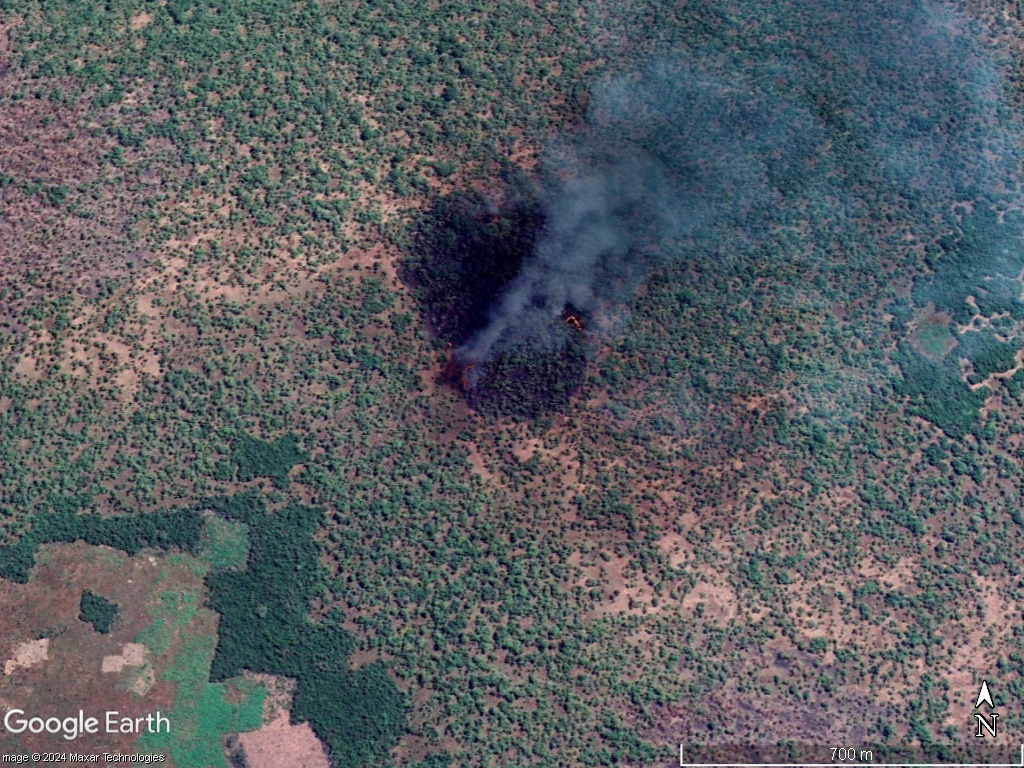
\includegraphics[width=0.8\textwidth,height=\textheight]{thicket-fire.jpg}

}

\caption{\label{fig-map}Distribution of the Itigi-Sumbu Thicket}

\end{figure}%

\begin{itemize}
\tightlist
\item
  \textbf{Immigration pressure} --- particularly around Lakes Mweru
  Wantipa and Tanganyika, driven by the fishing industry
\end{itemize}

A critical vulnerability is the ecosystem's \textbf{very low capacity to
regenerate} after clearance. Cultivation breaks down the specialised
duricrust soil structure, making recovery effectively impossible even
under protection.

\begin{center}\rule{0.5\linewidth}{0.5pt}\end{center}

\subsection{Protected Areas}\label{protected-areas}

Less than a quarter of the ecosystem falls within strictly protected
areas. In Zambia, \textbf{Mweru Wantipa National Park} and
\textbf{Nsumbu National Park} (IUCN Category II) have demonstrably
slowed thicket loss. By contrast, the largest remnants of the ecosystem
in Tanzania's Singida and Tabora regions have \textbf{no strict
protection}, and deforestation there is increasing sharply.

\begin{center}\rule{0.5\linewidth}{0.5pt}\end{center}

\subsection{Risk Assessment Summary}\label{risk-assessment-summary}

\begin{longtable}[]{@{}
  >{\raggedright\arraybackslash}p{(\columnwidth - 4\tabcolsep) * \real{0.3784}}
  >{\raggedright\arraybackslash}p{(\columnwidth - 4\tabcolsep) * \real{0.1486}}
  >{\raggedright\arraybackslash}p{(\columnwidth - 4\tabcolsep) * \real{0.4730}}@{}}
\caption{IUCN Red List assessment outcomes by criterion}\tabularnewline
\toprule\noalign{}
\begin{minipage}[b]{\linewidth}\raggedright
Criterion
\end{minipage} & \begin{minipage}[b]{\linewidth}\raggedright
Category
\end{minipage} & \begin{minipage}[b]{\linewidth}\raggedright
Notes
\end{minipage} \\
\midrule\noalign{}
\endfirsthead
\toprule\noalign{}
\begin{minipage}[b]{\linewidth}\raggedright
Criterion
\end{minipage} & \begin{minipage}[b]{\linewidth}\raggedright
Category
\end{minipage} & \begin{minipage}[b]{\linewidth}\raggedright
Notes
\end{minipage} \\
\midrule\noalign{}
\endhead
\bottomrule\noalign{}
\endlastfoot
A1 (past 50-yr decline) & \textbf{EN} & \textasciitilde59\% loss
1973--2023 \\
A2a (future 50-yr decline) & \textbf{EN--CR} & 53--94\% projected
loss \\
A2b (any 50-yr period) & \textbf{EN--CR} & 65--94\% decline
1986--2036 \\
A3 (historical decline) & \textbf{VU--EN} & Likely \textgreater70\%
since pre-industrial \\
B1 (Extent of Occurrence) & LC & EOO \textgreater110,000 km² \\
B2 (Area of Occupancy) & LC & 104--229 grid cells \\
C \& D (biotic degradation) & DD & Insufficient data \\
E (quantitative analysis) & DD & Not yet conducted \\
\end{longtable}

\textbf{Overall assessment: Endangered (EN), plausibly EN--CR}

\begin{center}\rule{0.5\linewidth}{0.5pt}\end{center}

\subsection{Conservation Priorities}\label{conservation-priorities}

\begin{enumerate}
\def\labelenumi{\arabic{enumi}.}
\tightlist
\item
  \textbf{Establish protected areas} in Tanzania's Singida and Tabora
  regions, where the largest intact blocks remain unprotected
\item
  \textbf{Halt further soil degradation} --- cleared areas are unlikely
  to recover
\item
  \textbf{Further ecological research} --- species inventories, soil
  dynamics, and comparison of Tanzania vs.~Zambia sub-types are needed
\item
  \textbf{Monitor deforestation} using continued remote sensing to
  detect further acceleration
\end{enumerate}

\begin{quote}
The intensity of agricultural encroachment and the urgency of
conservation efforts will define the future of this ecosystem --- one
that, once lost, cannot be recovered.
\end{quote}



\end{document}
